% reward_flow.tex — GRPO reward signal flow diagram
% Standalone TikZ figure; can also be \input{} into main.tex
% Compile: pdflatex reward_flow.tex
\documentclass[tikz,border=4pt]{standalone}

\usepackage{tikz}
\usepackage{amsmath}   % for \dfrac
\usetikzlibrary{arrows.meta, positioning, shapes.geometric, calc, fit}

% ── Shared colour palette ────────────────────────────────────────────────────
\definecolor{ModelOrange}  {RGB}{220, 130,  50}
\definecolor{ModelBg}      {RGB}{255, 235, 210}
\definecolor{CompBlue}     {RGB}{ 50, 110, 190}
\definecolor{CompBg}       {RGB}{215, 232, 255}
\definecolor{DataGreen}    {RGB}{ 55, 150,  90}
\definecolor{DataBg}       {RGB}{218, 245, 225}
\definecolor{ArrowDark}    {RGB}{ 60,  60,  80}
\definecolor{FormulaBg}    {RGB}{250, 250, 235}
\definecolor{FormulaBorder}{RGB}{180, 170,  80}

% ── Node styles ─────────────────────────────────────────────────────────────
\tikzset{
  % LLM / model node
  modelnode/.style={
    rectangle, rounded corners=6pt,
    fill=ModelBg, draw=ModelOrange, line width=1.1pt,
    text=ModelOrange, font=\bfseries\scriptsize,
    inner sep=6pt, minimum width=1.7cm, minimum height=0.65cm,
    align=center
  },
  % Computation step node
  compnode/.style={
    rectangle, rounded corners=5pt,
    fill=CompBg, draw=CompBlue, line width=0.9pt,
    text=CompBlue, font=\scriptsize,
    inner sep=5pt, minimum width=1.9cm, minimum height=0.60cm,
    align=center
  },
  % Data / intermediate-result node
  datanode/.style={
    rectangle, rounded corners=5pt,
    fill=DataBg, draw=DataGreen, line width=0.9pt,
    text=DataGreen, font=\scriptsize,
    inner sep=5pt, minimum width=1.7cm, minimum height=0.58cm,
    align=center
  },
  % Formula box
  formulabox/.style={
    rectangle, rounded corners=3pt,
    fill=FormulaBg, draw=FormulaBorder, line width=0.7pt,
    text=black, font=\tiny,
    inner sep=4pt, align=center
  },
  % Arrow
  flowarrow/.style={
    ->, >=Stealth, line width=0.85pt, color=ArrowDark
  },
  % Arrow label
  arrowlabel/.style={
    font=\tiny, text=ArrowDark, midway, above, inner sep=1.5pt
  }
}

\begin{document}
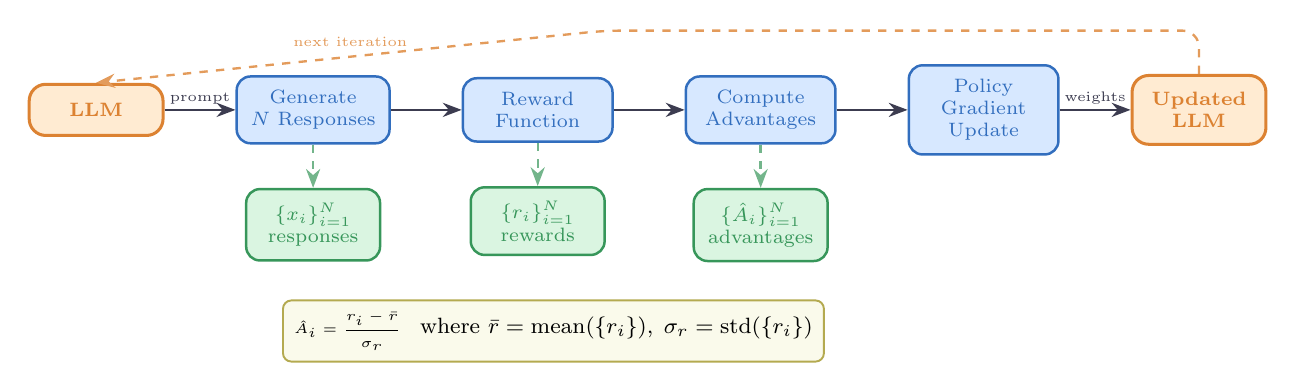
\begin{tikzpicture}[node distance=0.55cm and 0.45cm]

  % ── Pipeline nodes (horizontal, left → right) ─────────────────────────────

  % 1. LLM (input)
  \node[modelnode] (llm_in) {LLM};

  % 2. Generate N responses
  \node[compnode, right=0.9cm of llm_in] (gen) {Generate\\$N$ Responses};

  % 3. Reward function
  \node[compnode, right=0.9cm of gen] (rf) {Reward\\Function};

  % 4. Compute advantages
  \node[compnode, right=0.9cm of rf] (adv) {Compute\\Advantages};

  % 5. Policy gradient update
  \node[compnode, right=0.9cm of adv] (pg) {Policy\\Gradient\\Update};

  % 6. Updated LLM (output)
  \node[modelnode, right=0.9cm of pg] (llm_out) {Updated\\LLM};

  % ── Data annotations (below each node) ───────────────────────────────────

  % Responses annotation
  \node[datanode, below=0.55cm of gen] (resp_data)
        {$\{x_i\}_{i=1}^{N}$\\responses};

  % Rewards annotation
  \node[datanode, below=0.55cm of rf] (rew_data)
        {$\{r_i\}_{i=1}^{N}$\\rewards};

  % Advantages annotation
  \node[datanode, below=0.55cm of adv] (adv_data)
        {$\{\hat{A}_i\}_{i=1}^{N}$\\advantages};

  % ── Arrows between pipeline nodes ────────────────────────────────────────
  \draw[flowarrow] (llm_in.east)  -- node[arrowlabel]{prompt} (gen.west);
  \draw[flowarrow] (gen.east)     -- (rf.west);
  \draw[flowarrow] (rf.east)      -- (adv.west);
  \draw[flowarrow] (adv.east)     -- (pg.west);
  \draw[flowarrow] (pg.east)      -- node[arrowlabel]{weights} (llm_out.west);

  % ── Arrows from pipeline nodes to data annotations ────────────────────────
  \draw[flowarrow, dashed, color=DataGreen!70]
        (gen.south)  -- (resp_data.north);
  \draw[flowarrow, dashed, color=DataGreen!70]
        (rf.south)   -- (rew_data.north);
  \draw[flowarrow, dashed, color=DataGreen!70]
        (adv.south)  -- (adv_data.north);

  % ── Key formula (below centre) ────────────────────────────────────────────
  \node[formulabox,
        below=0.55cm of rew_data,
        xshift=0.2cm]
  (formula)
  {%
    $\hat{A}_i = \dfrac{r_i - \bar{r}}{\sigma_r}$%
    \quad
    \footnotesize where $\bar{r}=\mathrm{mean}(\{r_i\}),\;\sigma_r=\mathrm{std}(\{r_i\})$%
  };

  % ── Feedback loop arrow (Updated LLM → LLM) ───────────────────────────────
  % Arc above the pipeline
  \draw[flowarrow, color=ModelOrange!80, dashed, rounded corners=6pt]
        (llm_out.north)
        -- ++(0, 0.55)
        -- ++(-7.55, 0)
        -- (llm_in.north)
        node[midway, above, font=\tiny, text=ModelOrange!80] {next iteration};

\end{tikzpicture}
\end{document}
